\chapter{CSA} \label{ch:CSA}
The CSA is currently the most commonly used encryption algorithm in DVB for 
encryption of video-streams. There are two versions of the DVB-CSA, CSA1 and 
CSA2, where the key-length is the only difference between them 
\citep[p. 23]{DVBScene:2013}. 

The CSA uses a combination of a block cipher, taking an input of a 64-bit block, 
and a stream cipher. Both of the ciphers use the same key, so that the entire 
system uses the same key \citep[pp. 271--272]{WeiLi:2007}. This means that the 
complete algorithm would break if the key would be recovered. Using the same key 
does on the other hand allow us to easily change the key at regular intervals. 

CSA has been the official scrambling method for DVB since may 1994. CSA was 
to be easily implemented in hardware and hard to implement in software to make 
reverse-engineering difficult \citep{DVBScene:2013}.

%\section{History} \label{sec:History}
%CSA was largely kept secret until 2002, possibly since it was designed to be hard to reverse-engineered. The patent papers gave some hints of the layout, but important details like the layout of the S-boxes remained secret. Without the S-boxes, free implementations of the algorithm were out of question. Initially, CSA was to remain implemented in hardware only, but software implementations were found on the internet, which made it possible to analyze the entire solution.

%In 2002 FreeDec was released, implementing CSA in software. Though released as binary only, disassembly revealed the missing details and allowed reimplementation of the algorithm in higher-level programming languages. \Warning[source]{Is this relevant, and you need another source than Wikipedia}

%With CSA now publicly known in its entirety, cryptanalysts started looking for weaknesses.

\begin{figure}
  \begin{center}
    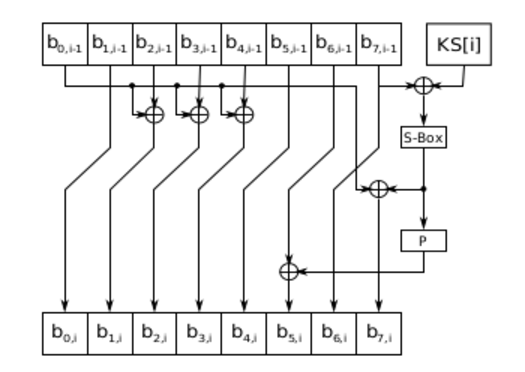
\includegraphics{blockcipher}
  \end{center}
  \caption{Image from \citet[pp. 49]{Breaking:2012}}
  \label{fig:blockcipher}
\end{figure}

\section{Why do we need a new standard?}
The DVB-CSA standard offers short-term protection (it assumes content is viewed 
in real time and not stored). Due to the development of how content is viewed 
during recent years, we now primarily need to be able to distribute content 
across homes. This means that the focus needs to be moved from securing delivery 
to securing content. \citep{Farncombe}

Another thing to bear in mind is the fact that more CPU-based units, such as 
smart-phones, tablets and computers are used to access contents now more than 
ever. In order to allow for descrambling on CPU-based units, a software-friendly 
scrambling algorithm might be needed.

\section{Layout of the CSA}
The CSA consists a block cipher and a stream cipher connected in sequence 
\citep[p. 271]{WeiLi:2007}. The block cipher reads 64-bit blocks of data, which 
is then run in Cipher Block Chaining-mode. The block cipher processes these 
blocks of data in 56 rounds. The output of this is sent to the stream cipher 
where additional encoding is performed. The first block of data sent from the 
block cipher to the stream cipher is used as an IV for the stream cipher, and is 
not encoded in this phase. \citep{DVBAnalysis:2006}

\section{Security}
One of the problems associated with CW distribution is the fact that CW sharing 
has become rather common \citep{Farncombe}. This is possibly due to the fact that
the CW is sent in the clear between the smart card and the STB, meaning that a 
user might grab the clear CW during transmission and redistribute it over the 
internet. This has become a financial problem for content distributors, since 
people stop paying for the content which they are watching.

One way of dealing with CW sharing is to decode the encrypted CW on the CI 
system, and then encrypt it once again on the CI, before sending it to the STB. 
The latter key is setup between the CI system and the STB  through a one time
sychronization. This means that users are not able to grab the clear CW and 
redistribute it. \citep[pp. 12--13]{HIS:2011}

Another security issue that you need to think of when designing the hardware, to 
prevent content theft, is to make sure that no contacts are ever accessible from 
the top layer of the circuit board. This is due to the fact that people would be 
able to connect hardware to the board and download the material that way, if they
were. \Warning[Source]{Except from Patrik Lantto}

We also need to be aware of people trying to break the algorithm through forced 
ways as well as CW sharing and hardware methods of stealing content.
%\subsection{Breaking the CSA}

There are a few standard ways to try when you want to break a cipher. 
Those are the brute force approach, known-plaintext attacks, chosen plaintext 
attacks and birthday attacks \citep[pp. 31-34]{Schneier:2003}. You choose what 
method to use depending on what the ciphers look like. I will not discuss all 
of them, but I will talk about the most relevant ones here.

\subsection{Brute force}
The CSA uses a key consisting of 64-bits, which gives us 18.5 Quintillion 
possible keys (Quintillion is $10^{18}$). But byte 3 and 7 are often used as 
parity bytes in CA systems which leads to only 48 bits being used in the key 
\citep{Breaking:2012}. This can be seen in figure \ref{fig:blockcipher}. 48 bits 
on other hand leads to $2^{48}$ combinations, which corresponds to 281 trillion 
possible keys (Trillion is $10^{12}$). Testing a million keys per second is about 
what is possible through on a modern x86 processor using software methods
\Warning[Todo]{How did I get this number?}, which means it would take roughly 
3258 days to force brake the keys. That is roughly 8.8 years.

Moreover, systems need to change the key at least every 120 seconds \citep{Simpson:2009} and most systems issues new keys every 10-120 second \citep{Wirt:2004}.

It is possible to use dedicated hardware and FPGA implementations to speed this 
up, using hardware accelerations and other methods. But even if we would be able 
to scan through 2.8 trillion keys per second, precisely allowing us to be certain
to find the key in two minutes, we could just change the key more often. As such,
the brute force method of obtaining the key is not a feasible option.

%\subsection{Bit slicing}
%The stream cipher part of CSA is prone to bit slicing, a software implementation 
%technique that allows decryption of many blocks, or the same block with many 
%different keys, at the same time. This significantly speeds up a brute force 
%search implemented in software, although the factor is too low to make a real-time 
%attack practical.

%The block cipher part is harder to bit slice, as the S-boxes involved are too large 
%(8x8) to be efficiently implemented using logical operations, a prerequisite for bit 
%slicing to be more efficient than a regular implementation.

